\chapter{Digital Signal Processing } \label{chap:hdl}

In order to implement the USBL system, a custom digital signal processing system has been implemented to compute in real-time the time differences of arrival of the acoustic signal arriving to the hydrophone array. The system was implemented in a FPGA-based platform and included in a previous signal processing system that determines the time of arrival of an encoded acoustic signal by implementing an efficient time-domain cross correlation. 

This chapter introduces the process to calculate the time differences of arrival by combining the results of the cross-correlation with the differences of phase between the signals received by the different hydrophones.

\section{TDoA Estimation}

To improve the determination of the time difference of arrival between the hydrophones, the implemented signal processing system calculates the difference of phase between the received signals. As the distance between hydrophones, i.e. the baseline, is always larger than the wavelength of the acoustic signals used, the phase alone is not sufficient to determine the time difference of arrival. Time-domain correlation is thus combined with the phase difference calculation to remove the ambiguity and obtain a time difference of arrival with a time resolution that is far beyond the sampling period used in the digital signal processing system.

When the information about the time of arrival of a signal is available, it is relatively easy to estimate the distance between the transmitter and the receiver since there can be a direct conversion between them. However, when dealing with phase differences, there is no exact time notion, so it is necessary to start by defining a reference point. 

Considering sinusoidal signals, when we have an array with four hydrophones spatially placed to form a 3D layout, the signal that is arriving to each  hydrophone in different times consequently have different phases. However, since sinusoidal signals are periodic, this means that for different signal periods the same phase value is observed, i.e. the phase is ambiguous \ref{fig:phasediff}. In this illustration, $\alpha$ represents the observable phase difference of hydrophone $H_4$ to the reference point $H_1$. However, the actual time difference which is intended to obtain, $\Delta t_4$, is one period of the signal, $\lambda$, added to the observable phase $\alpha$.

\begin{figure}[!htbp]
	\centering
	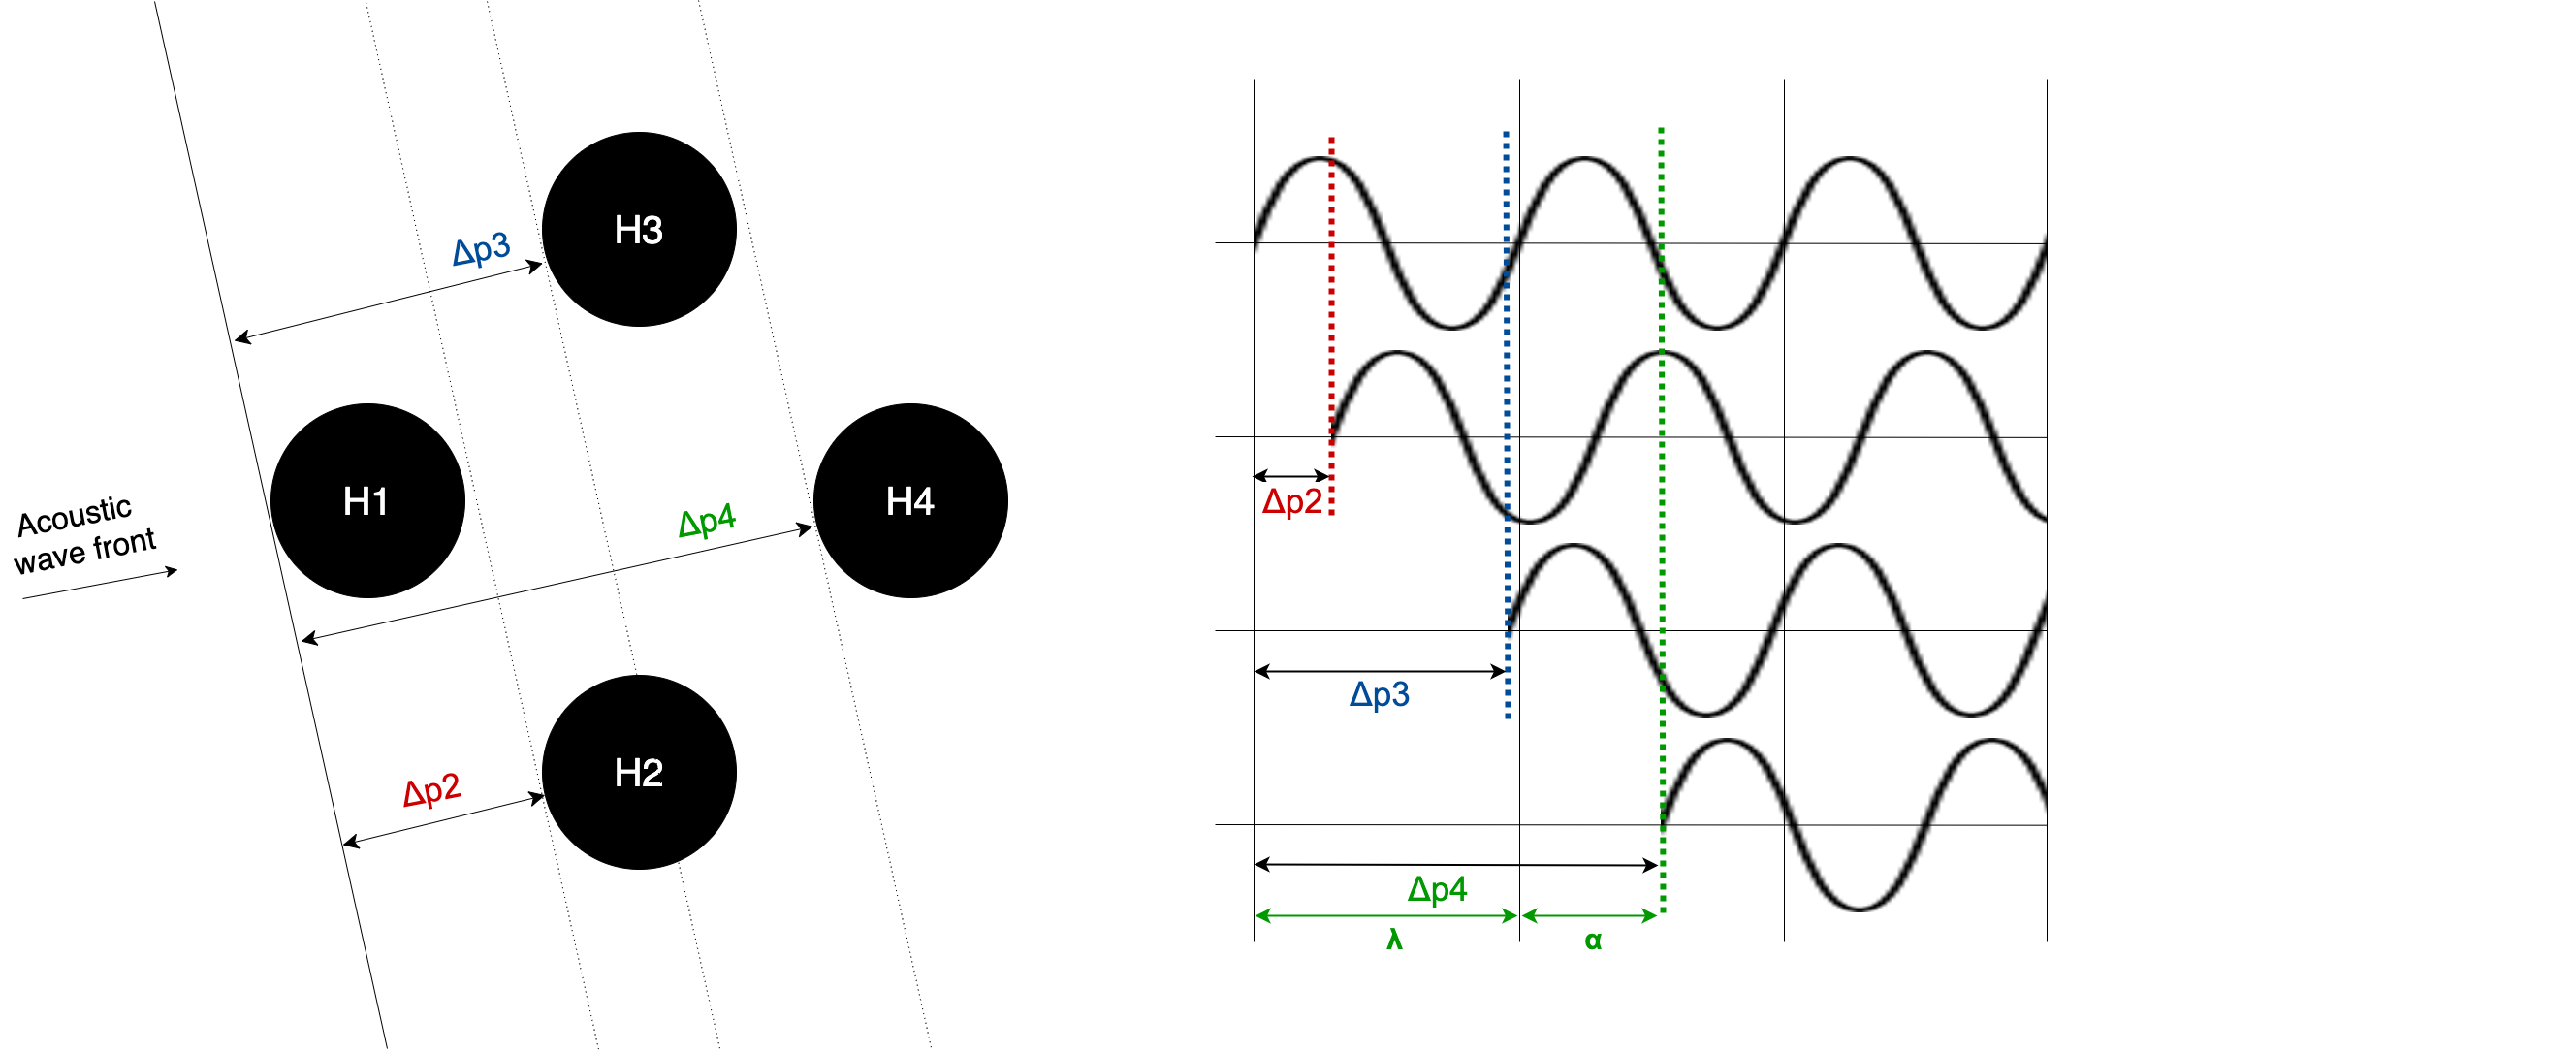
\includegraphics[width=1.2\textwidth]{figures/phase-diff}
	\caption{Phase difference to reference point and phase ambiguity}
	\label{fig:phasediff}
\end{figure}

For this reason, it is crucial to consider that the phase difference is given by the obtained phase value added by the number of periods ahead from the considered reference period.

In the system under study, the transmitted signal is a pure sine wave with a frequency of 24.4 $kHz$. The corresponding signal period is $T = \frac{1}{24400} $ seconds which, considering the typical underwater acoustic speed $c_s$ equal to 1500 $m/s$, the wavelength is approximately equal to $\lambda = \frac{T}{c_s} = 6.1 cm$. Having this into consideration, after obtaining the time of arrival to each hydrophone given by the cross correlation instances, besides the reference one, it is possible to conclude if the phase shift is superior to one period by analyzing if the time difference is greater than the duration of one period $T$. In figure \ref{fig:phasediff}, each mentioned time difference $\Delta t_2$, $\Delta t_3$ and $\Delta t_4$, between $H_1$ and $H_2$, $H_3$ and $H_4$ is converted to the corresponding phase differences.

One possibility to solve phase ambiguity in this system would be to place the four hydrophones with a baseline spacing inferior to $\frac{1}{2}$ of a wavelength, since the maximum reached by phase difference is 180 degrees. This way it would be possible to immediately deduce the phase difference since it would always be contained in one period. However, positioning the hydrophones closer together leads to smaller  values, causing an increase on the estimation error due to varying environment conditions (briefly enumerated in \ref{subsec: acoustic-channel}). Additionally, since the hydrophones to be used in this system have a corresponding diameter of roughly half of a wavelength, they would not allow to execute the mentioned configuration and so this possibility will not be contemplated.

In order to compensate this phase ambiguity, a simple relation was developed which allows to calculate the absolute time difference between the moment a signal is received by hydrophone A, $T_A$, and when the same signal is received by a further hydrophone B, $T_B$. Figure \ref{fig:ambiguity} illustrates this association, where the represented sinusoidal waves correspond to the same signal arriving at hydrophones A and B. 

\begin{figure}[!htbp]
	\centering
	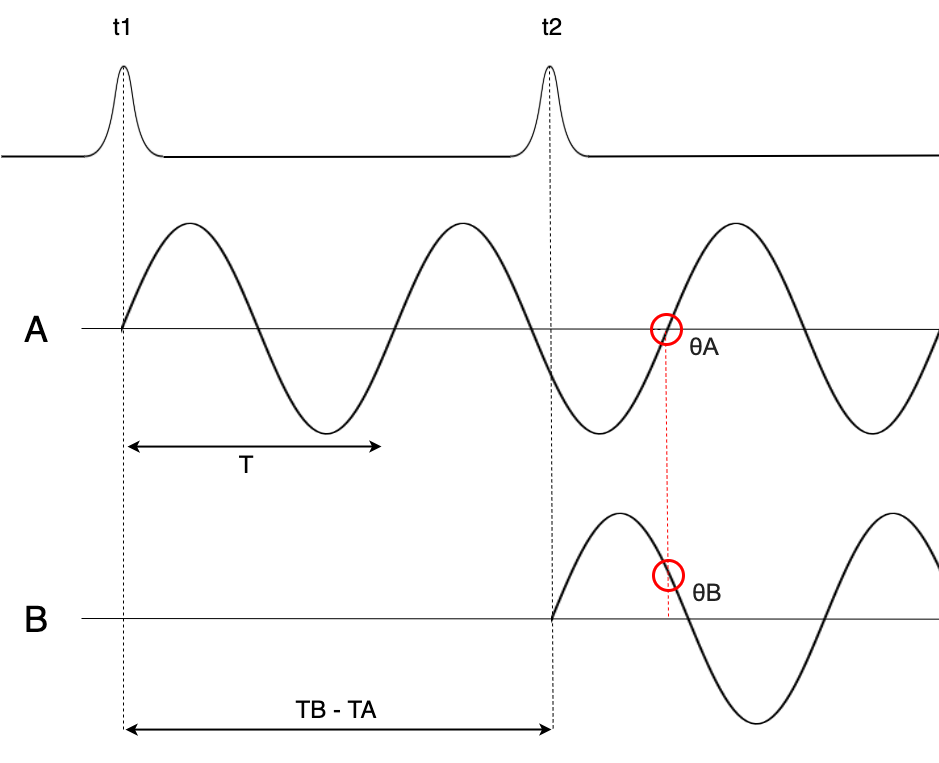
\includegraphics[width=0.6\textwidth]{figures/ambiguity}
	\captionsetup{justification=centering,margin=2cm}
	\caption{Ambiguity correction through correlation and phase difference}
	\label{fig:ambiguity}
\end{figure}

This correspondence uses the time stamps obtained by the correlation peaks combined with the calculated phase difference, that is determined in parallel, so that the measurement is more accurate. Equation (\ref{eq:phase-amb}) translates this relation, where $t_1$ and $t_2$ are the correlation peaks obtained from the signal arriving at hydrophone A and B, respectively, and so by rounding for the next integer number the difference between the correlation peaks, $t_2 - t_1$, we will obtain in which period, $T$, of signal in A will the signal in B arrive. Then the measurement is improved by subtracting a phase difference, $\theta_B - \theta_A$, so that the instant at which the signal is detected in hydrophone B can be defined. 

\begin{eqnarray}
	& T_B - T_A = round(\frac{t_2-t_1}{T}) - (\theta_B - \theta_A)
	\label{eq:phase-amb}
\end{eqnarray}

\section{HDL Module Architecture} \label{subchap:HDL module}

In a previous dissertation project \cite{afonso-thesis}, a signal processing system has been implemented to determine the time difference of arrival of an acoustic signal to a set of 4 hydrophones. This system is based on the transmission of a known binary sequence modulated in PSK (Phase Shift Keying) and the detection of the signal received by performing an efficient time-domain cross-correlation between the signals received at each hydrophone and the transmitted signal. The system was intended to determine the 3D position of an acoustic source in a confined structured space, where the 4 hydrophones were distanced a few meters between them. The implemented correlation process allow to obtain the time of arrival of the sound wave with a timing resolution equal to one sampling period that corresponds to a distance resolution approximately equal to 6 mm, which has been considered enough for the spacial accuracy of the 3D positioning system.

The current work intends to enhance that system to improve the accuracy of the calculation of the time differences of arrival. This is achieved by computing in real time the phase differences between the signals arriving to each hydrophone and combining that with the time of arrival calculated by the correlation process. The objective of this system is to implement a Ultra-Short Base Line (USBL) underwater localization system to estimate the 3D angle of arrival of the acoustic signal, for integration in a small Autonomous Underwater Vehicle (AUV). Due to the relatively small size of the AUV, the 4 hydrophones will have to be separated by the maximum of a few tens of centimeters. Therefore, the maximum resolution in distance that is possible to obtain with the correlation process alone is not enough for accurately determining the angle of arrival. Preliminary experimental results have showed that, with the phase analysis combined to the cross-correlation, the time differences may be obtained with an accuracy corresponding to a distance below one millimeter. 

To implement this process, that acoustic source transmits a sinusoidal signal with a know fixed frequency (24.41 kHz) after the BPSK encoded signal used by the correlation process. The phase analysis mechanism makes use of this signal which is know to appear a fixed time after the detection of the encoded signal.

\subsection{Module Components}

The overall system is composed by four main functional blocks, represented in \ref{fig:module-all}. The hydrophone array, composed by hydrophones $i$ with $i=\{1,2,3,4\}$, receives the signals in each sensor and sends them to an Analog to Digital Converter (ADC). The generated digital signals are then input of a module based on a Hilbert transform, which converts the real signals to their complex representation. These are then multiplexed so each pair of real, $Re_i$, and imaginary, $Im_i$, components are input in a CORDIC \cite{cordic-def} block, responsible for computing the signal's phase, $phase_i$. Afterwards, the phase differences $phdiff_{ij}$ are calculated for all the combinations of two hydrophones and finally they are averaged in order to obtain a more stable phase difference, $\Delta phase_{ij}$.

The module receives a global clock and reset which are connected to all registers, as well as an enable signal which allows the sub modules to capture new inputs and release the outputs synchronically.

\begin{figure}[!htbp]
	\makebox[\textwidth][c]{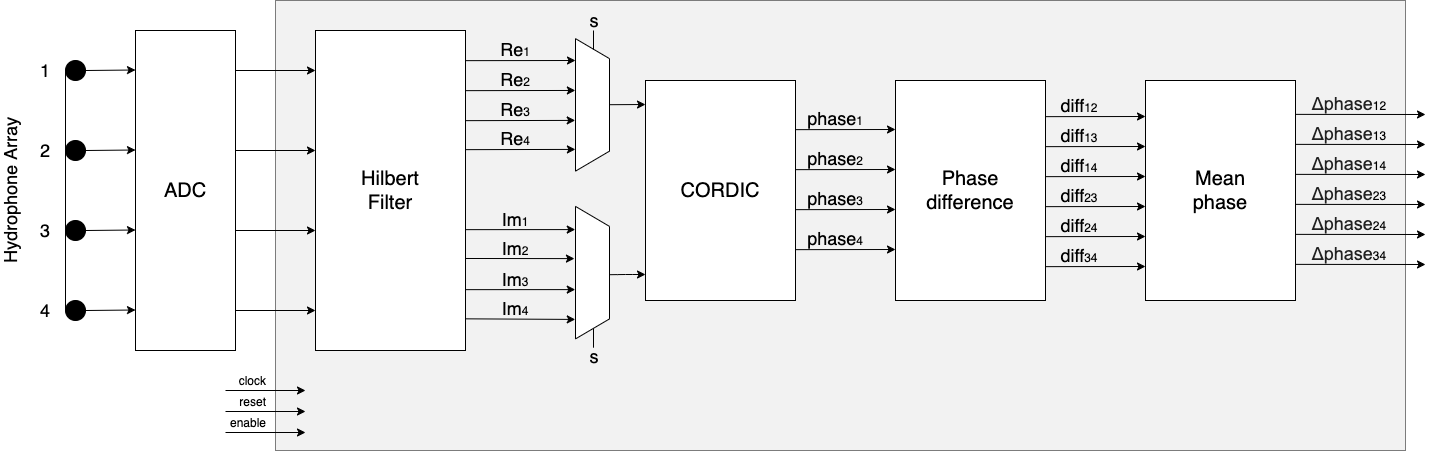
\includegraphics[width=1\textwidth]{figures/hdl-diagram-all}}
	\captionsetup{justification=centering,margin=2cm}
	\caption{Top level architecture}
	\label{fig:module-all}
\end{figure}

The sampling frequency of the input signals is 244 kHz and the whole digital circuit works with a global clock signal equal to 125 MHz. Thus, there are 512 clock cycles available between each two arriving signal samples and, as the calculations to perform are simple, these are more than enough to originate the outputs, therefore this architecture does not involve time constraints. Instead, it focuses on minimizing the used area since it is part of a complex system that already uses a substantial part of the FPGA resources.

In order to describe the efforts to minimize the used area, all module sub components are detailed next, namely the Hilbert filter, CORDIC, Phase difference and Mean phase.

\subsubsection{Hilbert Filter}

The signals coming from the ADC are purely real so they need to be converted to their analytic representation. This is achieved by using a module based on a Hilbert FIR filter, which derives the complex representation by comprehending the original real signal and its Hilbert transform. 

The Hilbert transform definition is given by (\ref{eq:hilbert_integral}) \cite{hilbert-def}, where $x(t)$ is the original signal and $P$ is the Cauchy principal value.

\begin{eqnarray}
	H(x)(t) = \frac{1}{\pi} \ P \int_{-\infty}^{\infty}\frac{x(\tau)}{t-\tau}d\tau
	\label{eq:hilbert_integral}
\end{eqnarray}

An 8-th order Hilbert FIR filter was designed using the Matlab function \textit{designfilt} and has only 4 non-zero coefficients. Although this will provide an inaccurate calculation for the instantaneous phase of the input signals along the signal period, it has been observed with Matlab simulations that this approximation will be enough for obtain an averaged phase difference within a few degrees. Nevertheless, the length of the Hilbert filter can be easily increased without a significant impact in the digital design complexity.

The 8th order Hilbert filters coefficients $a_k, k=1,...,7$ respect an odd anti-symmetry, i.e. $a_{1} = - a_{7}$ and $a_{3} = - a_{5}$. Thus, the imaginary and real components of the input signal $x_i$ are obtained by following equations (\ref{eq:hilbert_imeq}) and (\ref{eq:hilbert_reeq}). 

\begin{eqnarray}
	&Imag_0 = a_{1} \ x_{-1} +a_{3} \ x_{-3} + a_{5} \ x_{-5} + a_{7} \ x_{-7} \\
	\label{eq:hilbert_imeq}
	&Real_0 = x_{-4} 
	\label{eq:hilbert_reeq}
\end{eqnarray}

In order to implement this filter, the most common approach is to use a chain of registers that integrate multiple adders and multipliers, so that the calculations take less clock cycles to obtain a valid result, similarly to the work in \cite{hilbert-fpga}. However, since the goal of this implementation is to minimize area, then an alternative approach was formulated which uses only one multiplier and one adder. As can be observed in the filter equation, all odd samples need to be multiplied by a coefficient and summed with each other. Therefore, by using a circular shifting register chain \ref{fig:hilbert-chai} for each arriving signal, it is possible to position each of the buffer chain's samples in register $x_8$, which is used for external calculations.

\begin{figure}[!htbp]
	\makebox[\textwidth][c]{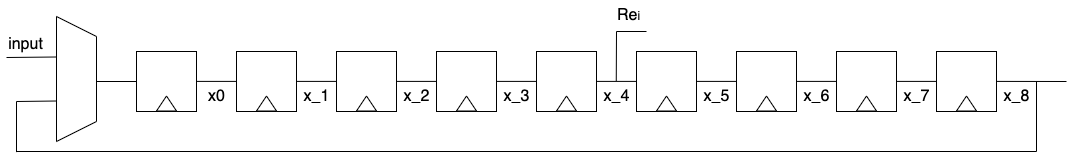
\includegraphics[width=0.9\textwidth]{figures/hilbert-filt-chain}}
	\captionsetup{justification=centering,margin=2cm}
	\caption{Hilbert Filter circular shifting register chain}
	\label{fig:hilbert-chai}
\end{figure}

In a more comprehensive view, the register chains $HF_{Ci}$ are integrated with the remaining block elements as represented in \ref{fig:hilbert-all}. The four shift-register chains receive four signals as input and output the real and imaginary components, $Real_i$ and $Imag_i$, for each of them.

\begin{figure}[!htbp]
	\makebox[\textwidth][c]{\includegraphics[width=0.9\textwidth]{figures/hilbert-filt-all}}
	\captionsetup{justification=centering,margin=2cm}
	\caption{Hilbert Filter block diagram}
	\label{fig:hilbert-all}
\end{figure}

The implementation contains a series of design decisions that lead to decreased area occupation, presented as follows :

\begin{itemize}
	\item The four register chains are multiplexed so that the module needs only one multiplier and one adder to calculate the Hilbert transform for all signals;
	
	\item Since the coefficients have odd symmetric pairs, then only two variables and their symmetric value are needed, which will be referred as $c_a = a_7 = - a_1$ and $c_b = a_5 = - a_3$. For even samples, associated with coefficients equal to zero, a controller unit is responsible for skipping the multiplication, which saves energy. For odd samples, the control unit alternates between the positive and negative coefficients to be multiplied. The control unit settings are summarized in table \ref{tab:coeffs-control-unit} for each register chain sample. 
	
	\begin{table}[!htbp] %use H to adjust
		\begin{center}
			\makebox[\textwidth]{
				\begin{tabular}{ c | c  c  }
					%\hline
					\toprule
					\multicolumn{1}{c|}{} & Multiplier Coefficient  & Adder mode\\	
					\midrule
					\multicolumn{1}{c|}{$a_0$} &  0 & -\\
					\midrule
					\multicolumn{1}{c|}{$a_1$} &  -$c_a$ & -\\
					\midrule
					\multicolumn{1}{c|}{$a_2$} &  0 & -\\
					\midrule
					\multicolumn{1}{c|}{$a_3$} &  -$c_b$ & -\\
					\midrule
					\multicolumn{1}{c|}{$a_4$} & 0 & +\\
					\midrule
					\multicolumn{1}{c|}{$a_5$} &  $c_b$ & +\\
					\midrule
					\multicolumn{1}{c|}{$a_6$} & 0 &+ \\
					\midrule
					\multicolumn{1}{c|}{$a_7$} &  $c_a$ & +\\
					\midrule
					\multicolumn{1}{c|}{$a_8$} & 0 &+ \\
					\bottomrule 
			\end{tabular}}
			\caption{Hilbert filter control unit settings for each processed sample with $c_a = 0.23932$ and $c_b = 0.62610$}
			\label{tab:coeffs-control-unit}
		\end{center}
	\end{table}
	
	\item The negative coefficients are achieved by subtracting the result of $a_{i} \ x_{-i}$, i.e. negating the adder, so only one adder block is necessary;
	
	\item A register is placed after the adder so that it interactively accumulates the value that is correspondent to the imaginary component $Im_i$ after the full chain circle shifting.
	
\end{itemize}

Having cleared the implementation details, it is possible to deduce that each $HF_{Ci}$ takes 9 clock cycles to be processed. Therefore, the entire calculation of the complex representation of the four input signals takes $9 \times 4$ clock cycles plus one additional cycle to update the outputs.

\subsubsection{CORDIC}

The CORDIC algorithm is used for real-time trigonometric and exponential calculations, as well as polar to rectangular conversions and vice-versa, using iterative vector rotations. 

The implemented CORDIC module has a sequential structure, as it occupies the least area, and it is responsible for receiving the real and imaginary components of a signal and calculating its phase. There are two possible modes of operation from which it is used the vectoring mode (VM), whose algorithm computes the magnitude and phase of the input vector $(x_0, y_0)$ from the x-axis \cite{cordic-def}. This is achieved by iteratively approximating the phase through angle microrotations of $\alpha_i = \ \pm atan(2^{-i})$ which are summed originating an approximated phase. The result is given in a 16 bit value, which is composed by 9 bits for the integer part and 7 bits that represent the fractional portion. 

The CORDIC iterations are expressed by (\ref{eq:cordic-iter-x}), (\ref{eq:cordic-iter-y}) and (\ref{eq:cordic-iter-z}) for $d_i$ belonging to \{-1,1\}.

\begin{eqnarray}
	& x_{i+1} = x_i - d_i \ 2^{-1} \ y_i
	\label{eq:cordic-iter-x}  \\
	& y_{i+1} = y_i + d_i \ 2^{-1} \ x_i
	\label{eq:cordic-iter-y} \\
	& z_{i+1} = z_i - d_i \ \alpha_i
	\label{eq:cordic-iter-z}
\end{eqnarray}

The CORDIC logic uses a 16 element ROM (Read-Only Memory) that stores the $atan(2^{-1})$ values required for the algorithm. Additionally, another sub component provides a binary counter that defines the number of performed iterations and it is also responsible for generating the address to access the ROM. 

Considering that the CORDIC module uses 16 clock cycles to run through the entire ROM and one additional cycle to update the outputs. Therefore, the design uses only one CORDIC module with multiplexed inputs so the process takes $17 \times 4$ plus one, to update the global outputs, in a total of 69 clock cycles.

\subsubsection{Phase Difference}

This sub module is responsible for computing the phase differences between the previously determined signals' phases, $phase_i$. For four inputs $phase_i$, it is generated the difference between all pairs of different hydrophones, $h_ih_j$: $h_1h_2$, $h_1h_3$, $h_1h_4$, $h_2h_3$, $h_2h_4$ and $h_3h_4$.

This is achieved using a single subtractor which has multiplexed inputs so that the calculations can be executed within the 512 clock cycles with only one block of hardware, instead of dedicated subtractor for each calculation. 

The result is given in a 16 bit value, which is composed by 10 bits for the integer part and 6 bits that represent the fractional portion. 

\subsubsection{Mean Phase}

Finally, the last module implements a moving window averaging filter, with a window size $N = 2^k$ configured by the parameter k, with values from 1 to 6. The final averaged phase differences are in the range [-180º,+180º], represented in 16 bits with 7 bits for the fractional part.

\subsection{Implementation Results}

The design was synthesized to a XILINX XC7Z010 Zynq \cite{xilinx-board} device and integrated in the digital signal processing system implemented in a Red Pitaya platform. Although this block is only a part of a more complex signal processing system that also includes the correlation calculators as described in \cite{afonso-thesis}, it occupies only 1216 flip-flops and 1462 Look-up tables, which represents a small fraction of the available FPGA resources. Besides, the sequential implementation of the Hilbert FIR filter and CORDIC module and the sharing of the modules among the four input signals has reduced the size of a previous preliminary implementation which used more than 10k flip-flops and 6k Loop-up tables.


%----------------------------------------------------------------------------------
\section{Doppler Effect}

The implemented process uses the information of the transmitted signal's operating frequency in order to compute the phase differences and determine the overall times of arrival. However, in real scenarios the environmental and the operational conditions will distort the frequency perceived by the receiver due to the relative movement between the acoustic source and the receiver.

In order to evaluate if the Doppler effect influences the system, it is possible to calculate the frequency deviation observed for a known relative speed between vehicles. Considering that the relative speed between the transmitter and the receiver is denoted as $relative\_speed$ and using a fixed sound speed, $c_s$, with a determined frequency of the transmitted signal, the relation (\ref{eq:doppler}) \cite{doppler-eq} can be established. 

\begin{eqnarray}
	&freq\_deviation = \frac{relative\_speed}{c_s} \times signal\_freq
	\label{eq:doppler}
\end{eqnarray}

Therefore, considering a maximum relative velocity between the transmitter and the receiver equal to $\pm \ 5 m/s$, this will impact in a frequency deviation perceived by the receiver equal to $\pm \ 81Hz$, which corresponds to a relative error of 0.33\% of the nominal frequency and approximately the same relative deviation for the period of the signal reaching the receiver. As the time differences calculated from the phase differences are directly proportional to the expected signal period, concerning the calculation of the time difference of arrival to different hidrophones, the Doppler effect has been considered negligible.

A way to prevent this deviation is to integrate a frequency detector which senses the relative navigation speed in real time and adapts the used frequency. This mechanism is not integrated in the present research work.